\documentclass[aspectratio=169]{beamer}
\usepackage[utf8]{inputenc}
\usepackage{transparent}
\usepackage{hyperref}
\usepackage{pgf}
\usepackage{dsfont}
\usepackage{algorithm}
\usepackage{algorithmic}
\usepackage{booktabs}

% here comes my custom theme for university of Bamberg

\logo{\pgfputat{\pgfxy(-1.25,4.25)}{\pgfbox[center,base]{\transparent{0.7} 
\includegraphics[width=.15\textwidth]{uni_bamberg.png}}}}


\newcommand{\nologo}{\setbeamertemplate{logo}{}} % command to set the logo to nothing
\newcommand{\biglogo}{\setbeamertemplate{logo}{\pgfputat{\pgfxy(-2,4)}{\pgfbox[center,base]{ 
\includegraphics[width=.24\textwidth]{uni_bamberg.png}}}}} 

% theming and colors and stuff
\usetheme[progressbar=frametitle, block = fill]{metropolis}
\definecolor{uniblau}{RGB}{4, 66, 119} %#044277
\definecolor{niceorange}{RGB}{255, 128, 0} %#ff8000
\definecolor{nicegray}{RGB}{221, 239, 244} %#ddeff4
\setbeamercolor{palette primary}{bg=uniblau, fg=white}
\setbeamercolor{normal text}{fg=uniblau, bg=white}
\setbeamercolor{itemize item}{fg=niceorange}
\setbeamercolor{itemize subitem}{fg=niceorange}
\setbeamercolor{itemize subsubitem}{fg=niceorange}
\setbeamercolor{enumerate item}{fg=niceorange}
\setbeamercolor{enumerate subitem}{fg=niceorange}
\setbeamercolor{enumerate subsubitem}{fg=niceorange}
\setbeamercolor{block body}{bg=nicegray}
\setbeamercolor{block title}{bg=niceorange,fg=white}
\renewcommand\UrlFont{\color{niceorange}\rmfamily}

% own commands for highlighting
\newcommand{\pop}[1]{{\color{niceorange}\textbf{#1}}}

\def\ps@titlepage{\setbeamertemplate{footline}{}}
\makeatletter
\setbeamertemplate{frame footer}{\tiny{xAI-Proj-M - Data Engineering - J.Amling }}

% custom python style

%title page
\title{Data Engineering  -- Background Removal}
\subtitle{Explainable Machine Learning - Deep Learning Life Cycle}
\author{Jonas Amling \and Baptiste Patrice Francis Bony \and Benedikt Markus Marsiske}
\institute{University of Bamberg}
\date{\today} 

\begin{document}
% titleframe
{\biglogo
	\setbeamertemplate{footline}{} 
	\begin{frame}{}
		\titlepage
	\end{frame}
}

\begin{frame}{Table of contents}
	\tableofcontents
\end{frame}


{\nologo
\section{Research Question}
	\begin{frame}{Research Question and Introduction}
	Our main Data Engineering Problems:
	\begin{itemize}
		\item Combining different datasets
		\item Different hand positions in different datasets
		\item Hands in different contexts in each dataset
		\pause
		\item	$\implies$ Reducing complexity of datasets is key
	\end{itemize}
	\pause
	Research Question: \pop{Does removing the background during the image preprocessing phase benefit the image classification task at hand?} 
	\end{frame}

\section{Data Engeneering Process}
	\begin{frame}{Test, Train and Validation Datasts}
	Combining Datasets of different sources:
	\begin{description}
		\item[Training Data] data combined from different datasets
		\begin{description}
			\item[custom] Self produced images 
			\item[cgi] Computer-generated images \footnote{\url{https://www.tensorflow.org/datasets/catalog/rock_paper_scissors}}
			\item[webcam] Existing Dataset from Kaggle (hands with bodies) \footnote{\url{https://www.kaggle.com/datasets/drgfreeman/rockpaperscissors}}
			\item[hands]	Existing Dataset from Kaggle (only hands from top) \footnote{\url{https://www.kaggle.com/datasets/glushko/rock-paper-scissors-dataset}}
		\end{description}
		\pause
		\item[Validation Data] Provided by the project (created by individual groups)
		\pause
		\item[Testing Data] Provided by the project (created by individual groups)
	\end{description}
	\end{frame}
	
	\begin{frame}{}
	\begin{columns}
	\column{0.2\textwidth}
	\begin{figure}
        \centering
        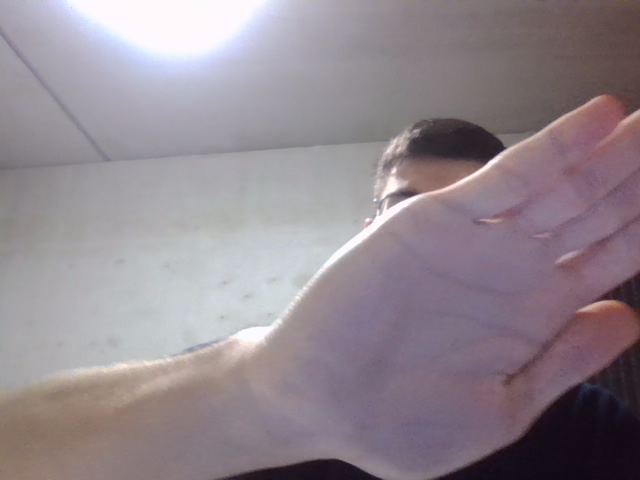
\includegraphics[width=0.5\textwidth]{img/test/4__bapt44.png}
   \end{figure}
   \begin{figure}
        \centering
        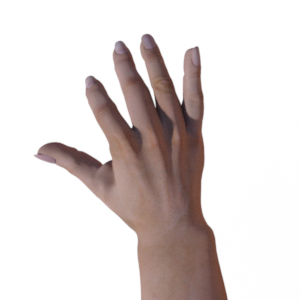
\includegraphics[width=0.5\textwidth]{img/test/3__paper01-095.png}
    \end{figure}  
    \begin{figure}
        \centering
        
\includegraphics[width=0.5\textwidth]{img/test/nasmi_203.png}
    \end{figure}  
    \begin{figure}
        \centering
        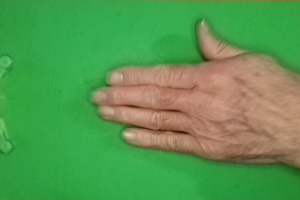
\includegraphics[width=0.5\textwidth]{img/test/2__4ZoU4nouZzb9G2MI.png}
    \end{figure}  
    
	\column{0.8\textwidth}
	\begin{figure}
        \centering
        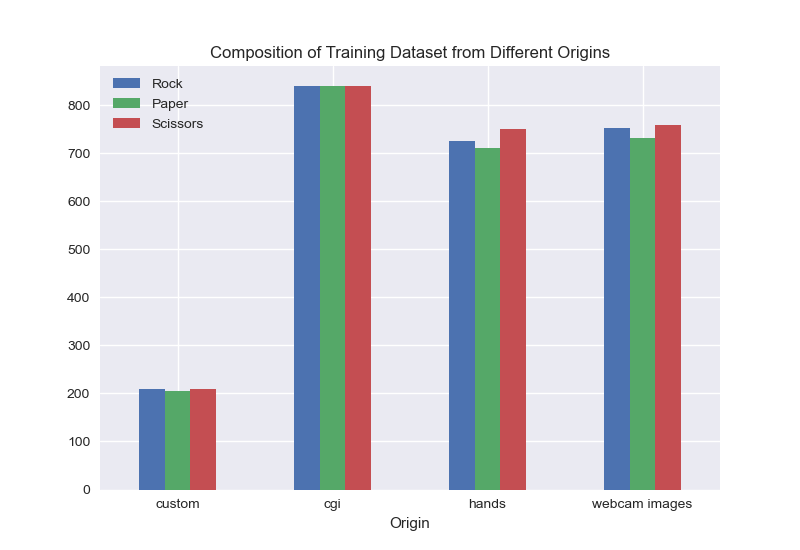
\includegraphics[width=\textwidth]{img/ds_analysis/train_ds.png}
        \caption{Distribution of individual Datasets}
    \end{figure} 
	\end{columns}
	\end{frame}
	
	
	\begin{frame}{Existing libraries I}
	Searching the WWW we found some interesting libraries:
	\begin{itemize}
		\item YOLO-Hand-Detection: find hand position in an image \footnote{https://github.com/cansik/yolo-hand-detection}
		\begin{itemize}
			\item[+] works on real life images, open source
			\item[-] not included in Python Package Index
		\end{itemize}
		\pause
		\item rembg: model that automatically removes image background \footnote{https://pypi.org/project/rembg/}
		\begin{itemize}
			\item[+] comes as library in Python Package Index 
			\item[-] not works in all cases, has some strange edge cases
		\end{itemize}
	\end{itemize}
	\end{frame}
	
	\begin{frame}{Existing libraries II}
	Searching the WWW we found some interesting libraries:
	\begin{itemize}
		\item MediaPipe Hands: generates a 3d hand model from a 2d image \footnote{https://google.github.io/mediapipe/solutions/hands.html} \cite{mediapipe}
		\begin{itemize}
			\item[+] works quite well and comes as library in Python Package Index 
			\item[-] developed by google
		\end{itemize}
	\end{itemize}
	\end{frame}
	
	\begin{frame}{The Preprocessor}
	Parameters for Image Processing:
	\begin{itemize}
		\item desired dimensions  of preprocessed image
		\item crop image, based on the hand position within the image (Mediapipe Hands)
		\item remove background (rembg)
		\item greyscale: convert images to one-channel greyscale images
	\end{itemize}
	\pause
	Preprocessing steps:
	\begin{enumerate}
	\item read image using cv2
	\item crop image based on bounding-box found with MediaPipe
	\item remove left over background using rembg library
	\item resize image and add padding if necessary
	\item use cv2 to convert images to greyscale
	\end{enumerate}
	\end{frame}
	
	
	\begin{frame}{Preprocessing Examples}

\begin{columns}[c]

    \begin{column}{.33\textwidth}
    \begin{figure}
        \centering
        
\includegraphics[width=0.6\textwidth]{img/test/nasmi_203.png}
        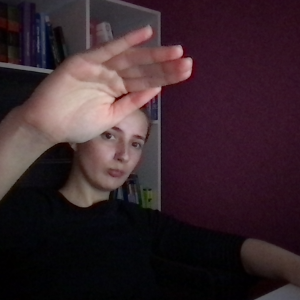
\includegraphics[width=0.6\textwidth]{img/test/nasmi_304.png}
        \caption{original}
    \end{figure}      
    \end{column}

    \begin{column}{.33\textwidth}
    \begin{figure}
        \centering
        
\includegraphics[width=0.6\textwidth]{img/cropped/nasmi_203.png}
        
        
\includegraphics[width=0.6\textwidth]{img/cropped/nasmi_304.png}
        \caption{cropped}
    \end{figure}
    \end{column}
   
    \begin{column}{.33\textwidth}
    \begin{figure}
        \centering
        
\includegraphics[width=0.6\textwidth]{img/rembg/nasmi_203.png}
        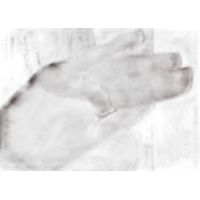
\includegraphics[width=0.6\textwidth]{img/rembg/nasmi_304.png}
        \caption{background removal}
    \end{figure}
    \end{column}
\end{columns}
\end{frame}

\begin{frame}{Parameter Selection for Preprocessor}
    Chosen parameters:
    \begin{description}
    \item[dimensions] (300,300), and again scaled down for model to (64,64)
    \item[crop images] True with a hand detection confidence of 0.1
    \item[remove background] False, since rembg did perform very poorly
    \item[greyscale] True
	 \end{description}        

\end{frame}

\begin{frame}{Media Pipe Hands Performance on Test Dataset}
	Evaluation the performance of hand detection with Mediapipe Hands with a confidence of 0.1

\begin{columns}[c]

    \begin{column}{.5\textwidth}
    \begin{table}[]
\begin{tabular}{@{}lllll@{}}
\toprule
\multicolumn{1}{c}{Origin} & Rock & Paper & Scissors & Total \\ \midrule
custom                     & 210  & 205   & 210      & 625   \\
cgi                        & 840  & 840   & 840      & 2520  \\
hands                      & 726  & 712   & 750      & 2188  \\
webcam                     & 752  & 733   & 760      & 2245  \\
Total                      & 2528 & 2490  & 2560     & 7578  \\ \bottomrule
\end{tabular}
\caption{Total number of images per origin}
\end{table}
    \end{column}

    \begin{column}{.5\textwidth}
    \begin{table}[]
\begin{tabular}{@{}lllll@{}}
\toprule
\multicolumn{1}{c}{Origin} & Rock   & Paper  & Scissors & Total  \\ \midrule
custom                     & 95.2\% & 90.7\% & 96.2\%   & 94.1\% \\
cgi                        & 89.0\% & 100\%  & 100\%    & 96.3\% \\
hands                      & 95.9\% & 99.6\% & 94.5\%   & 96.6\% \\
webcam                     & 93,5\% & 96.2\% & 91.8\%   & 93.8\% \\
Total                      & 92.8\% & 98.0\% & 95.6\%   & 95.5\% \\ \bottomrule
\end{tabular}
\caption{Percentage of detected hands in images}
\end{table}
    \end{column}
   
\end{columns}
\end{frame}

\section{Experiment}
	\begin{frame}{Same Model, Same Data, Different Processing, Same Result?}
	Here the basic Idea is to run the exactly same training simply with different preprocessed Datasets
	\begin{description}
    \item[H0]: \pop{Reagardless of the preprocessing used, the (blackbox) model should perform equally on the accuracy on the validation and test dataset in terms of accuracy }
	 \end{description}  
	 \begin{itemize}
		\item Preprocessor parameters are set as before, only difference is the use of cropping images based on Mediapipe Hands
		\item Model parameters: dropout probability: 0.5, no batch normalization, 100 epoches of training and a batch size of 64, Adam optimizer with learning-rate of 0.001 and CrossEntropy as criterion
		\item Compare the model performance on Train, Validation and Test Data after each 10 epoches of training
	\end{itemize}
	\end{frame}
	
	\begin{frame}{Schematic of Experiment Setup}
	\begin{figure}
        \centering
        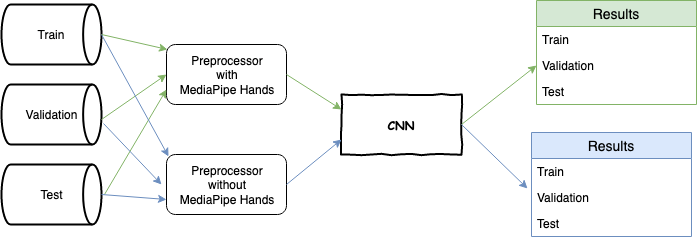
\includegraphics[width=0.9\textwidth]{img/experiment/Experiment_Setup.png}
        \caption{Experiment Setup}
    \end{figure}
	\end{frame}
	
	\begin{frame}{Results Training Data}
		\begin{columns}

    \column{0.6\textwidth}
    \begin{figure}
        \centering
        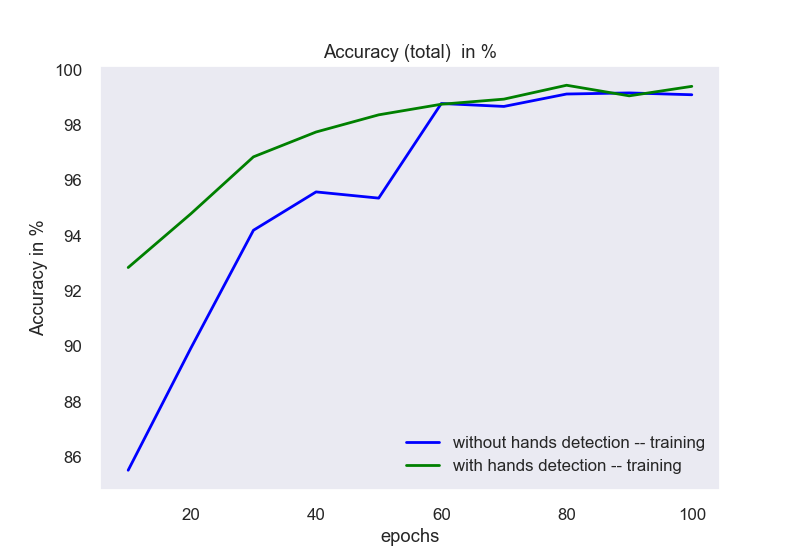
\includegraphics[width=1\textwidth]{img/experiment/model_comp_10steps__training_acc_total.png}
        \caption{Total Accuracy on Training Data}
    \end{figure}      

    \column{0.4\textwidth}
    \begin{figure}
        \centering
        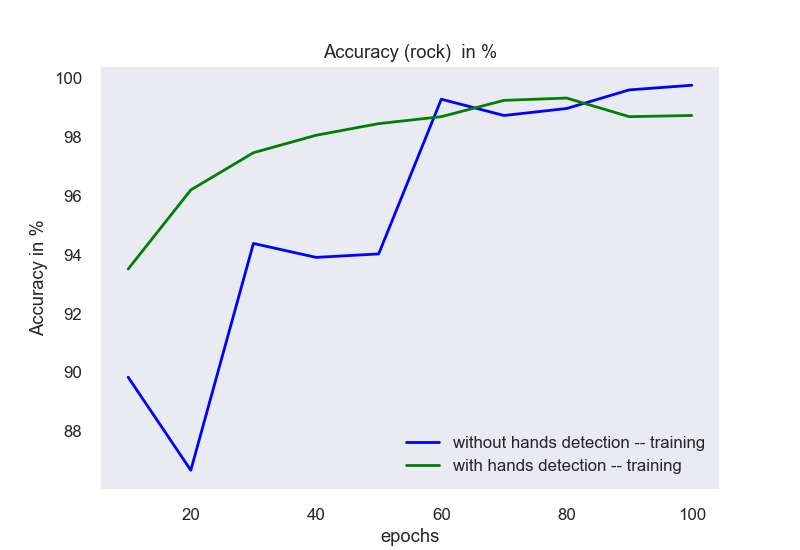
\includegraphics[width=0.6\textwidth]{img/experiment/model_comp_10steps__training_acc_rock.png}     
        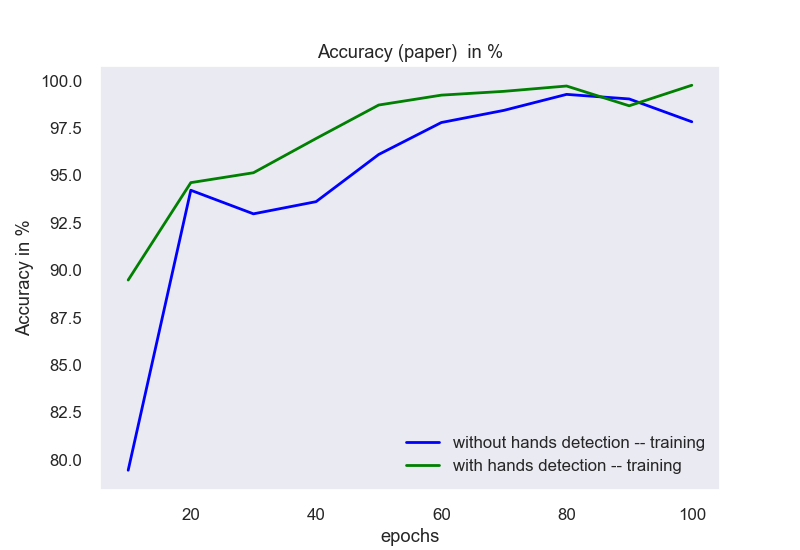
\includegraphics[width=0.6\textwidth]{img/experiment/model_comp_10steps__training_acc_paper.png}
        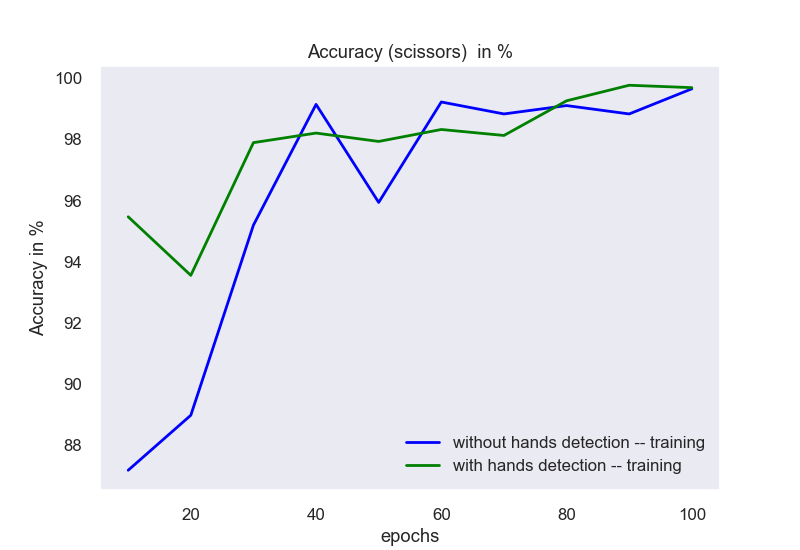
\includegraphics[width=0.6\textwidth]{img/experiment/model_comp_10steps__training_acc_scissors.png}
    \end{figure}
   
	\end{columns}
	\end{frame}
	
	\begin{frame}{Results Validation Data}
		\begin{columns}

    \column{0.6\textwidth}
    \begin{figure}
        \centering
        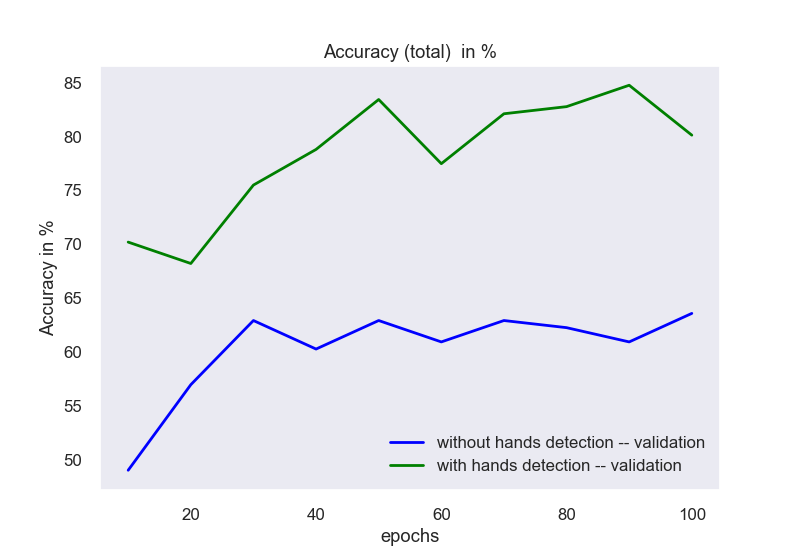
\includegraphics[width=1\textwidth]{img/experiment/model_comp_10steps__val_acc_total.png}
        \caption{Total Accuracy on Validation Data}
    \end{figure}      

    \column{0.4\textwidth}
    \begin{figure}
        \centering
        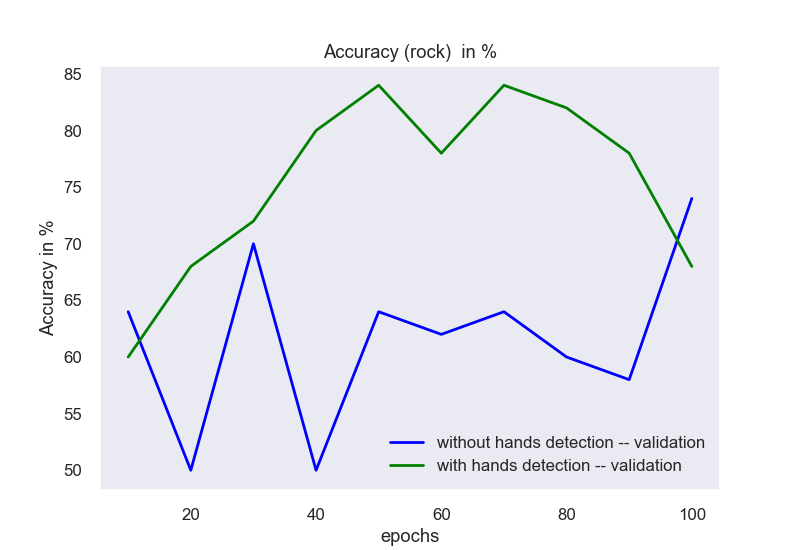
\includegraphics[width=0.6\textwidth]{img/experiment/model_comp_10steps__val_acc_rock.png}     
        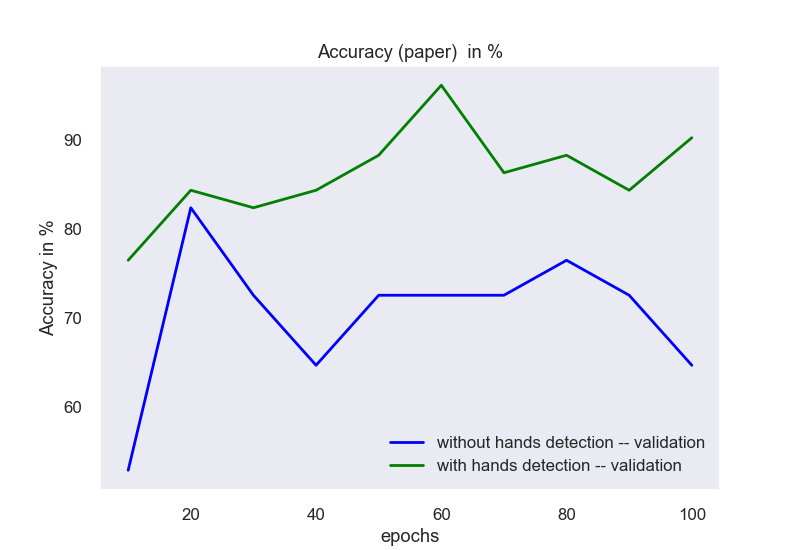
\includegraphics[width=0.6\textwidth]{img/experiment/model_comp_10steps__val_acc_paper.png}
        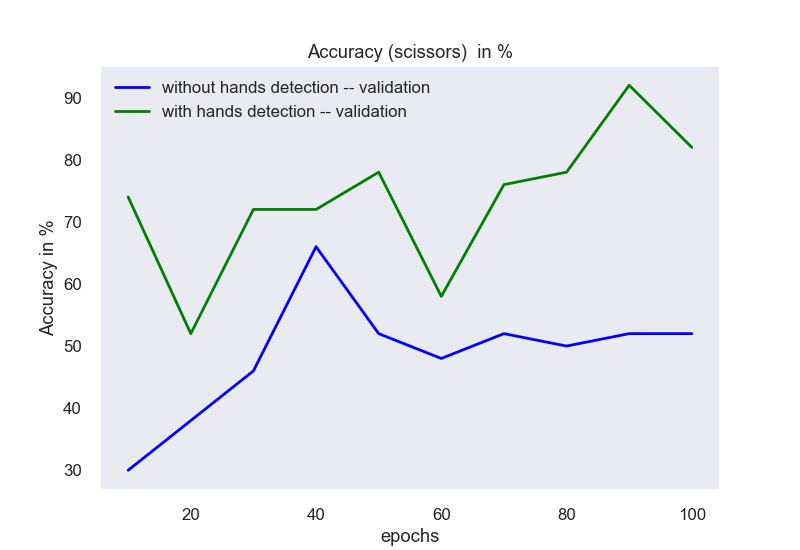
\includegraphics[width=0.6\textwidth]{img/experiment/model_comp_10steps__val_acc_scissors.png}
    \end{figure}
   
	\end{columns}
	\end{frame}
	
	\begin{frame}{Results Test Data}
		\begin{columns}

    \column{0.6\textwidth}
    \begin{figure}
        \centering
        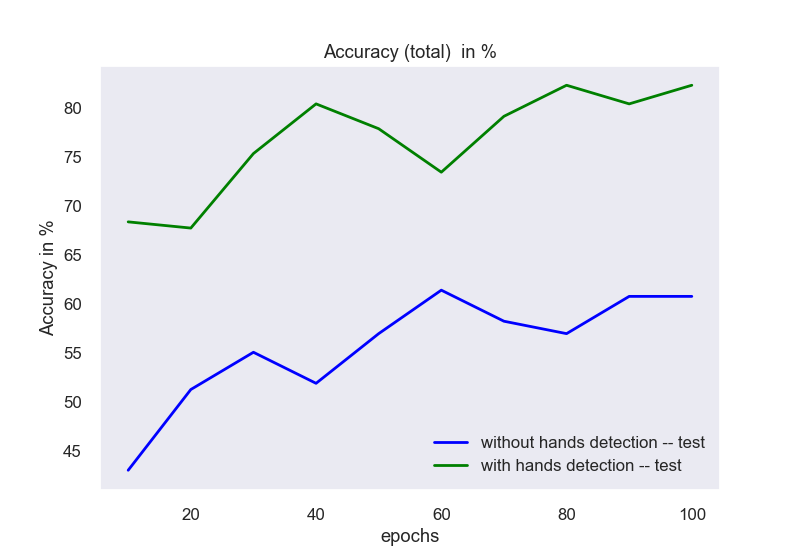
\includegraphics[width=1\textwidth]{img/experiment/model_comp_10steps__test_acc_total.png}
        \caption{Total Accuracy on Test Data}
    \end{figure}      

    \column{0.4\textwidth}
    \begin{figure}
        \centering
        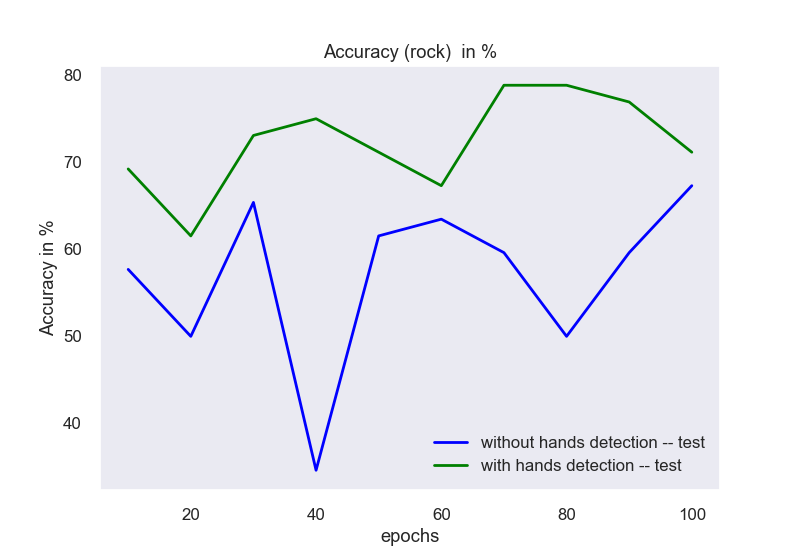
\includegraphics[width=0.6\textwidth]{img/experiment/model_comp_10steps__test_acc_rock.png}     
        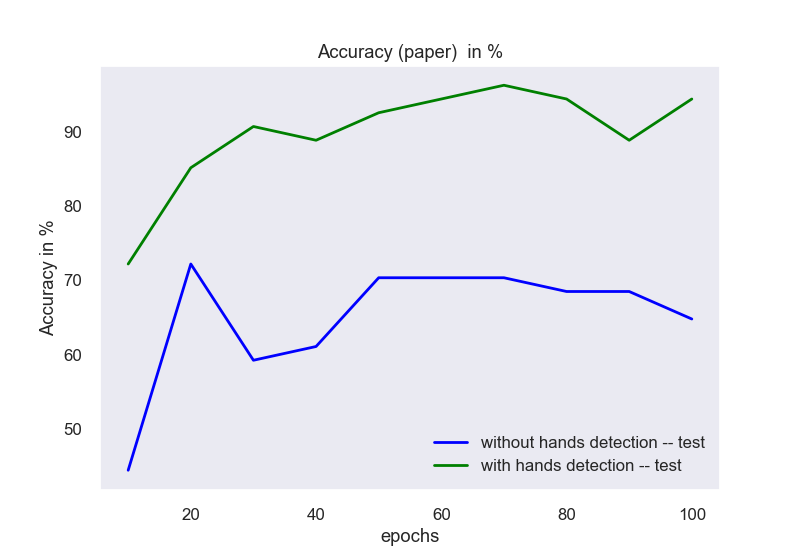
\includegraphics[width=0.6\textwidth]{img/experiment/model_comp_10steps__test_acc_paper.png}
        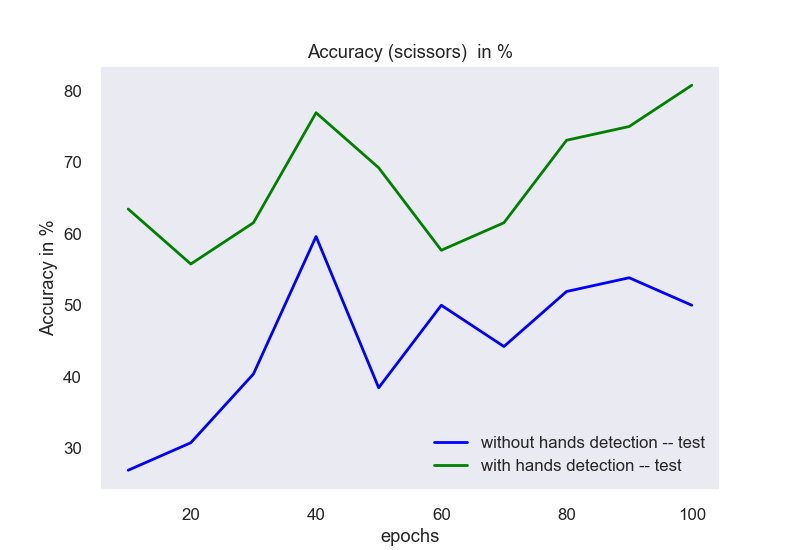
\includegraphics[width=0.6\textwidth]{img/experiment/model_comp_10steps__test_acc_scissors.png}
    \end{figure}
   
	\end{columns}
	\end{frame}


	\begin{frame}{Discussion}
	Results show that the preprocessor with image cropping based on Mediapipe Hands:
	\begin{itemize}
		\item Training Data: performed better at less training steps 
		\item Validation Data: performed better for each test model iteration
		\item Testing Data: performed better for each test model iteration
	\end{itemize}
	\pause
	$\implies$ \pop{H0} is probably \pop{not correct} and an alternative has to be considered
	\pause
	\newline
	$\implies$ based on the presented results it is to assume that \pop{reducing the complexity of the dataset} by removing the background (unimportant parts of the image) \pop{leads to better model performance}.
	
	\end{frame}
}


\appendix
{\nologo
	\begin{frame}[standout]
		Thank you!
	\end{frame}

    
	\begin{frame}[allowframebreaks]{References}
	
	\bibliographystyle{ieeetr}
  	\bibliography{references}
  	

	\end{frame}
}
\end{document}
